%====================================================================
%====================================================================
\appendix
\section*{Mixture Model for Random Graphs}
\subsection*{Mixture Model}
\frame{ \frametitle{Mixture Model} \pause
%==================================================================== 
  \paragraph{Discrete-valued latent labels:}
  each node $i$ belong to class $q$ with probability $\pi_q$:
  $$
  \{Z_i\}_i \mbox{ i.i.d.}, \qquad Z_i \sim \Mcal(1; \pibf)
  $$
  where $\pibf = (\pi_1, \dots \pi_K)$;

  \bigskip
  \paragraph{Observed edges:} $\{X_{ij}\}_{i,
    j}$ are conditionally independent given the $Z_i$'s:
  $$
  (X_{ij} \;|\; Z_i = k, Z_j = \ell) \sim f_{k\ell}(\cdot).
  $$
  where $f_{k\ell}(\cdot)$ is some parametric distribution
  $f_{k\ell}(x) = f(x; \gamma_{k\ell})$, e.g.
  $$
  (X_{ij}|Z_{ik}Z_{j\ell}=1) \sim \Bcal(\gamma_{k\ell})
  $$
  We denote   $\gammabf = \{\gamma_{k\ell}\}_{k, \ell}.$
  
  \bigskip
  \paragraph{Inference:} We need to estimate
  $$
  \thetabf = (\pibf, \gammabf)
  \qquad \text{and} \qquad
  P(Z_i | \Xbf)
  $$
  }

%==================================================================== 
\frame{ \frametitle{Illustration: A social network}
  \vspace{-1cm}\hspace{-1cm}
  \begin{tabular}{c}
    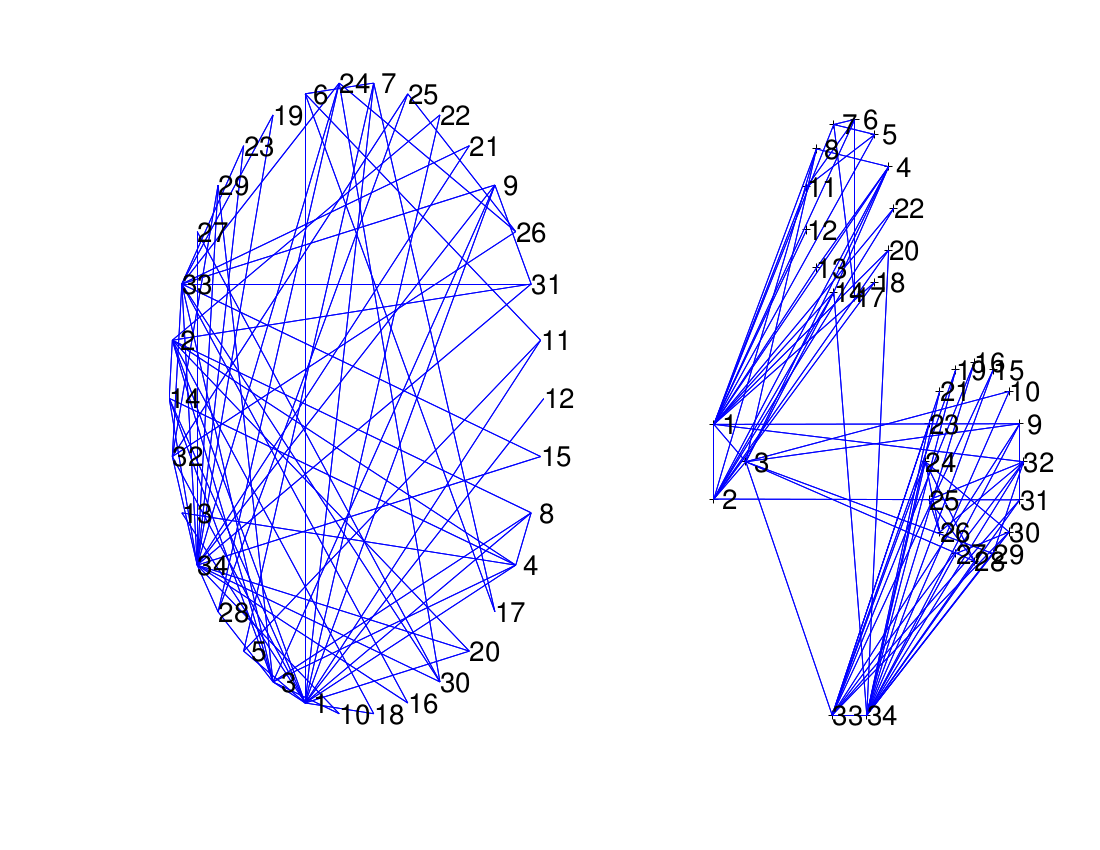
\epsfig{file = ../Figures/Karate-Graph.eps, clip=, width=3.5cm,
      height=10cm, angle=270}
    \\
    \\
    \begin{tabular}{cc}
      \begin{tabular}{p{.45\textwidth}}
        \paragraph{Data.} Social binary network of friendship within a
        sport club. \\
        \\
        \paragraph{Results.} 
        The split is recovered and the role of the leaders is underlined. 
      \end{tabular}
      &
      \begin{tabular}{p{.5\textwidth}}
        {\small
          \begin{tabular}{c|rrrr}
            & \multicolumn{4}{c}{$\widehat{\gamma}_{k\ell}$ (\%)} \\
            $k / \ell$ &  {1} & 2 & 3 &  4 \\
            \hline
            {1} &  {100} &   {53} &  {16} & {16} \\  
            {2} & - &  {12} & {0} & {7}  \\  
            3 & - & - & 8 & 73 \\
            4 & - & - & - & 100\\
            \hline
            $n\pi_{\ell}$        & 3 &  13       & 16    & 2     \\
          \end{tabular}
          }
      \end{tabular}
    \end{tabular}
  \end{tabular}
  }

%==================================================================== 
\subsection*{Variational Inference}
\frame{ \frametitle{Maximum likelihood inference}
%==================================================================== 
  \paragraph{Maximum likelihood estimate:} We are looking for
  $$
  \widehat{\thetabf} = \arg\max_{\thetabf} \log P(\Xbf; \thetabf)
  $$

  \paragraph{Incomplete data model:}
  \begin{itemize}
  \item The calculation of
    $$
    P(\Xbf; \thetabf) = \sum_{\Zbf} P(\Xbf, \Zbf; \thetabf)
    $$
    is not always possible since this sum typically involves $K^n$ terms.
  \item This of 
    $$
    P(\Xbf, \Zbf; \thetabf)
    $$
    is much easier ... except that {$\Zbf$ is unknown}.
  \end{itemize}
  }

%====================================================================
\subsection*{Variational approach}
\frame{ \frametitle{Variational approach}
%==================================================================== 
  \paragraph{Lower bound of the likelihood:}
  For any distribution $Q(\Zbf)$, we have [\refer{JGJ99,Jaa00}]
  \begin{eqnarray*}
    \log P(\Xbf) & \geq & \log P(\Xbf) - KL[Q(\Zbf); P(\Zbf|\Xbf)] \\
%     & = & \log P(\Xbf) - \int Q(\Zbf) \log Q(\Zbf) \dd\Zbf + \int
%     Q(\Zbf) \log \emphase{P(\Zbf |\Xbf)} \dd\Zbf \\   
%     & = & - \int Q(\Zbf) \log Q(\Zbf) \dd\Zbf + \int Q(\Zbf) \log
%     \emphase{P(\Xbf, \Zbf)} \dd\Zbf \\
    & = & \Hcal(Q) + \Esp_Q[\log P(\Xbf, \Zbf)].
  \end{eqnarray*}
  where
  \begin{eqnarray*}
    \Hcal(Q) & = & \int Q(\Zbf) \log Q(\Zbf) \dd\Zbf \\
    \Esp_Q[\log P(\Xbf, \Zbf)] & = & \int Q(\Zbf) \log \emphase{P(\Xbf, \Zbf)} \dd\Zbf
  \end{eqnarray*}
  }

%==================================================================== 
\frame{ \frametitle{Consequences}
  \paragraph{If $P(\Zbf|\Xbf)$ can be calculated}: taking $Q(\Zbf) =
  P(\Zbf|\Xbf)$ achieves the maximisation of $\log P(\Xbf)$ through
  this of
  $$
  \Esp_Q[\log P(\Xbf, \Zbf; \thetabf)].
  $$
  \emphase{$\rightarrow$} E-M algorithm for independent mixtures, hidden
  Markov models, etc. %[\refer{DLR77,MaP00,CMR05}].
  
  \bigskip\bigskip
  \paragraph{If $P(\Zbf|\Xbf)$ can not be calculated}: the best lower
  bound of $\log P(\Xbf)$ is obtained for
  $$
  Q^* = \arg\min_{Q \in \Qcal} KL[Q(\Zbf); P(\Zbf|\Xbf)]
  $$
  \emphase{$\rightarrow$} Mean-field approximation for random graphs.
  }

%====================================================================
\subsection*{Variational E-M}
\frame{ \frametitle{Variational E-M}
%==================================================================== 
  \paragraph{'Expectation' step (E-step):} calculate
  $$
  P(\Zbf|\Xbf; \thetabf)
  $$
  or its approximation
  $$
  Q^* = \arg\min_{Q \in \Qcal} KL[Q(\Zbf); P(\Zbf|\Xbf; \thetabf)].
  $$

  \bigskip
  \paragraph{Maximisation step (M-step):} estimate $\thetabf$ with
  $$
  \widehat{\thetabf} = \arg\max_{\thetabf} \Esp_Q[\log P(\Xbf, \Zbf; \thetabf)]
  $$
  which maximise $\log P(\Xbf)$ if $Q(\Zbf) = P(\Zbf|\Xbf)$, and its
  lower bound otherwise.
  }

%==================================================================== 
\frame{ \frametitle{Dependency structure}
  \begin{tabular}{c|c|c}
    \begin{tabular}{p{.28\textwidth}}
      \emphase{Graphical rep.:} \\ 
      $P(\Zbf) P(\Xbf|\Zbf)$
    \end{tabular}
    &
    \begin{tabular}{p{.28\textwidth}}
      \emphase{Moral graph}  \\
      (\refer{Lau96})
    \end{tabular}
    &
    \begin{tabular}{p{.28\textwidth}}
      \emphase{Cond. dependency:} \\ 
      $P(\Zbf|\Xbf)$
    \end{tabular}
    \\
    \hline
    & & \\
    \begin{tabular}{c}
      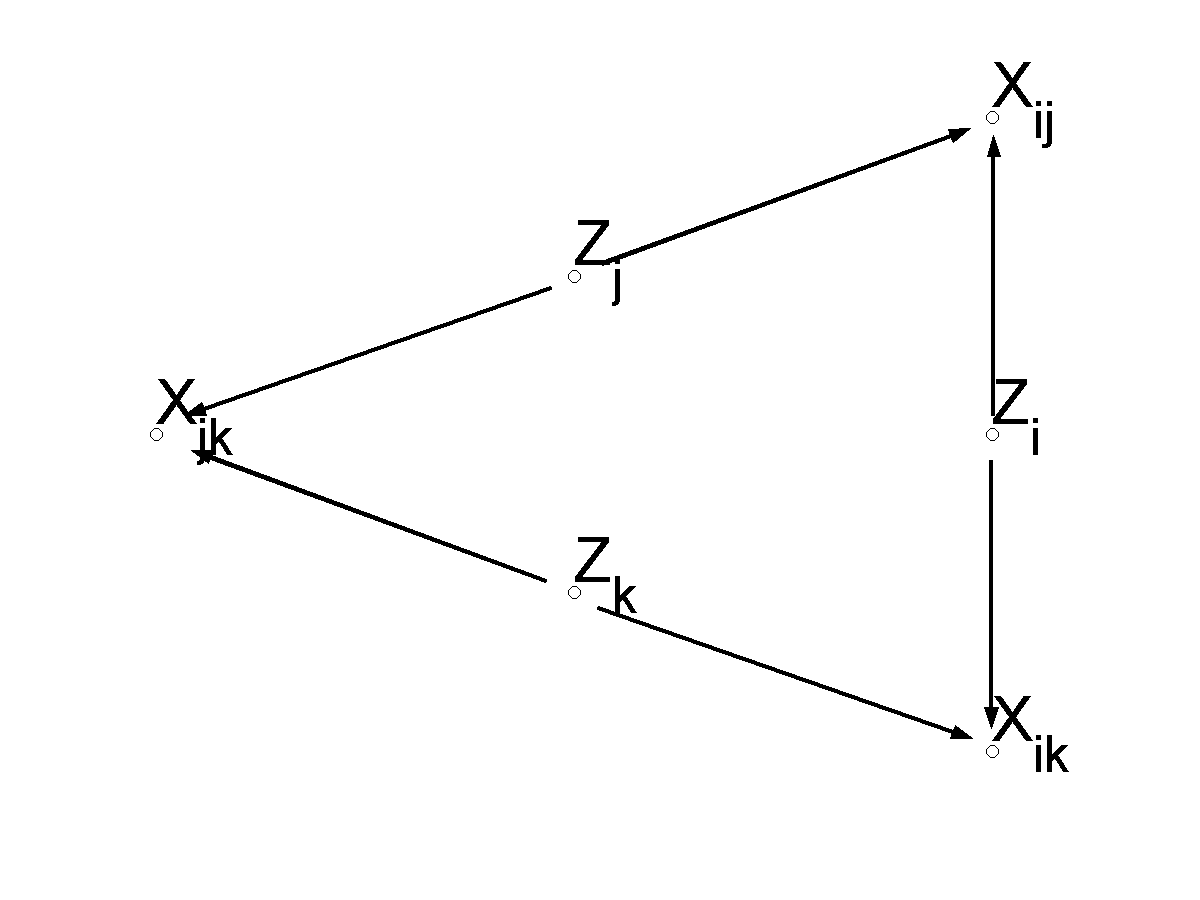
\epsfig{file=../Figures/FigNetworks-DepGraph,
      width=.25\textwidth, clip=} 
    \end{tabular}
    & 
    \begin{tabular}{c}
      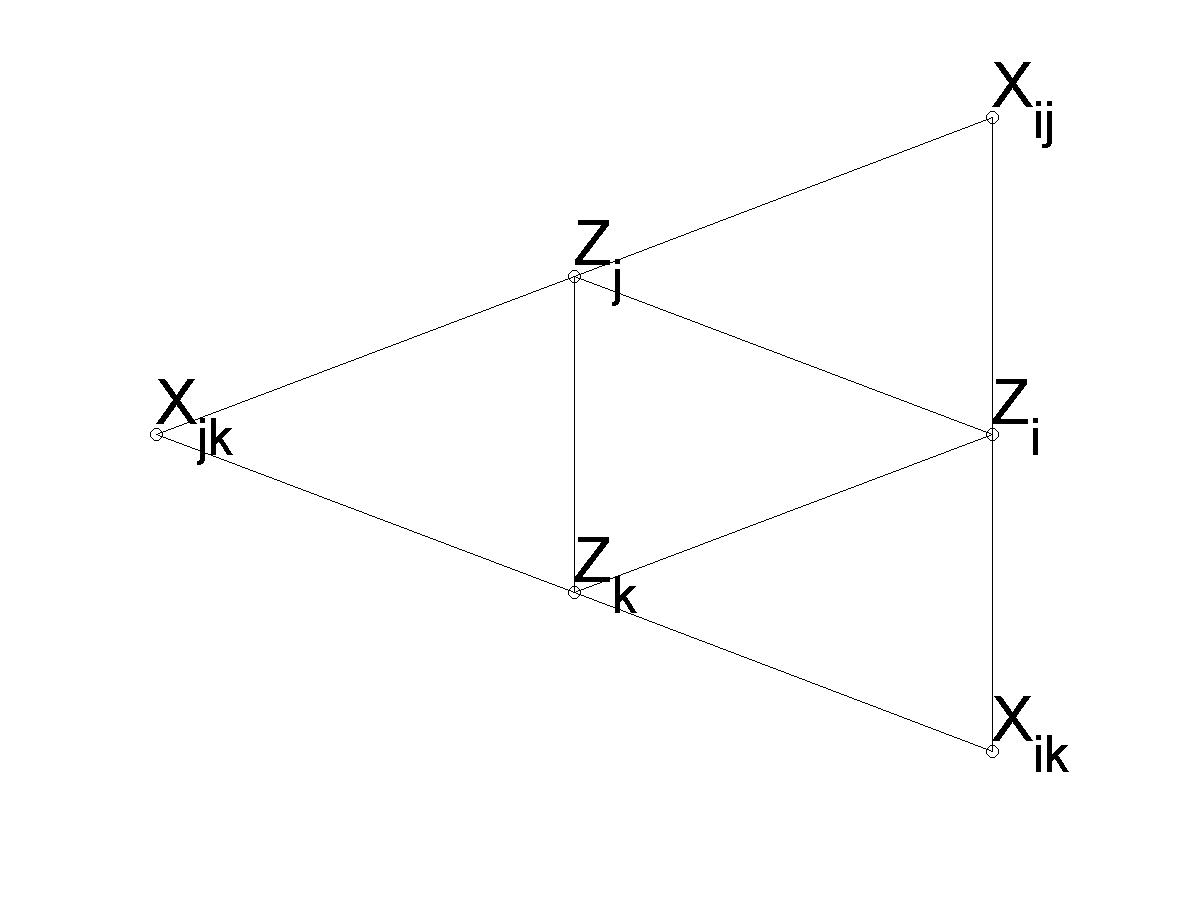
\epsfig{file=../Figures/FigNetworks-DepGraph-Moral,
      width=.25\textwidth, clip=}
    \end{tabular}
    & 
    \begin{tabular}{c}
      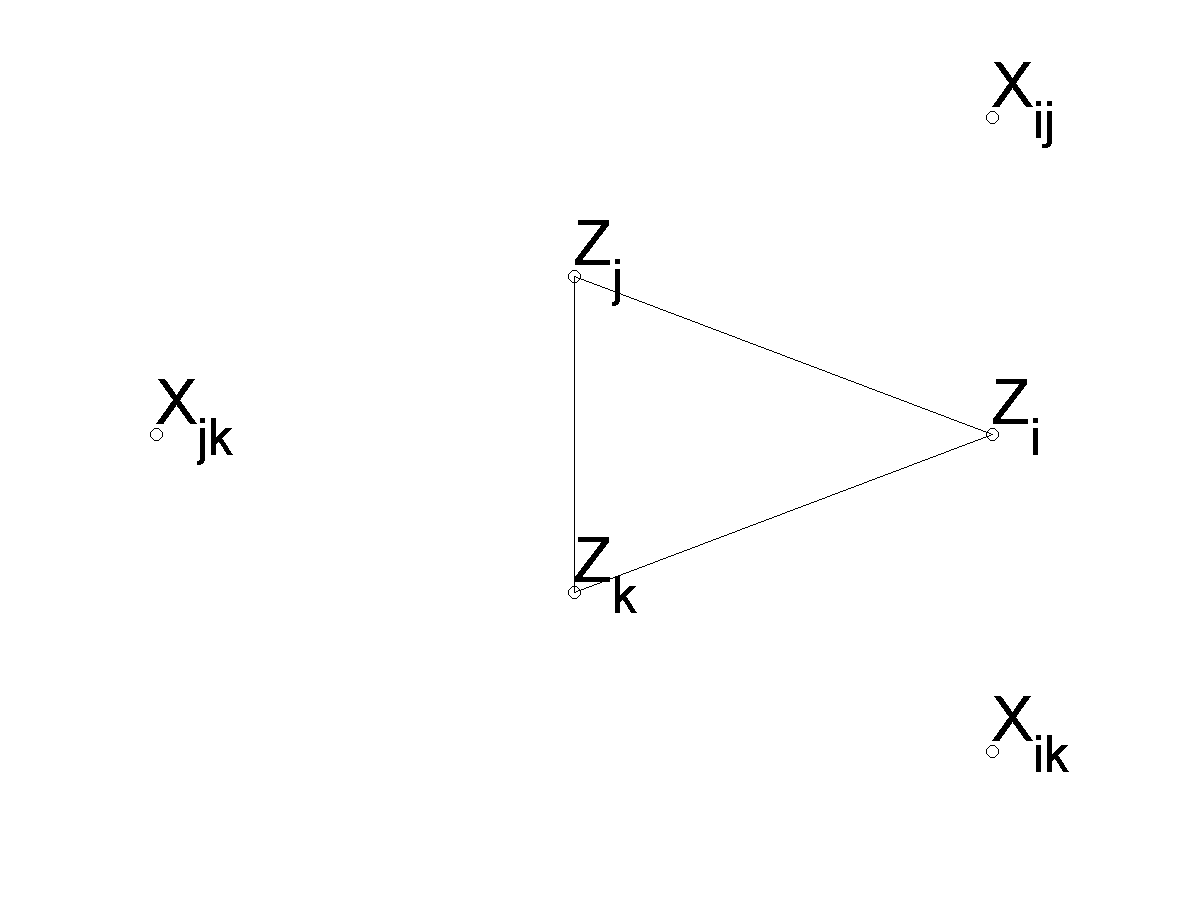
\epsfig{file=../Figures/FigNetworks-DepGraph-Conditional,
      width=.25\textwidth, clip=}
    \end{tabular} 
  \end{tabular}

  \bigskip\bigskip
  The conditional dependency of $\Zbf$ is a \emphase{clique} \\
  \emphase{$\rightarrow$} no factorisation can be hoped to calculate
  $P(\Xbf|\Zbf)$ \\
  \emphase{$\rightarrow$} $P(\Xbf|\Zbf)$ can {only be approximated}.
  }
%====================================================================
\subsection*{Inference}
\frame{ \frametitle{Likelihood}
%==================================================================== 
  \paragraph{Complete likelihood:}
  $$
  \log P(\Xbf, \Zbf) = \sum_{i, k} Z_{ik} \log \pi_k + \sum_{i, j}
  \sum_{k, \ell} Z_{ik} Z_{j\ell} \log f(X_{ij}; \gamma_{k\ell}).
  $$
   
  %\bigskip
   \paragraph{Completed likelihood:} 
   $$
   \Esp_Q[\log P(\Xbf, \Zbf)] = \sum_{i, k}
   \underset{\emphase{\normalsize
       \tau_{ik}}}{\underbrace{\Esp_Q[Z_{ik}]}} \log \pi_k + \sum_{i,
     j} \sum_{k, \ell} \Esp_Q[Z_{ik} Z_{j\ell}]  \log f(X_{ij};
   \gamma_{k\ell}). 
   $$
   
   ~\\
   \paragraph{M-step:} weighted version of the MLE.  
   }

%====================================================================
\frame{ \frametitle{Approximation of $P(\Zbf|\Xbf)$}
  \paragraph{Problem:}  
  We are looking for
  $$
  Q^* = \arg\min_{Q \in \Qcal} KL[Q(\Zbf); P(\Zbf|\Xbf)].
  $$

  \begin{itemize}
%   \item The optimum over all possible distributions is
%     \emphase{$Q^*(\Zbf) = P(\Zbf|\Xbf)$} ... which can no be
%     calculated.
  \item We restrict ourselves to the set of \emphase{factorisable
      distributions}:
    $$
    \Qcal = \left\{Q: Q(\Zbf) = \prod_i Q_i(Z_i) = \prod_i \prod_k
      \tau_{ik}^{Z_{ik}}\right\}. 
    $$
    $Q^*$ is characterised by the set of optimal parameters
    $\tau_{ik}^*$'s:
    $$
    \emphase{\tau_{ik}^* = \Esp_Q[Z_{ik}] \approx \Pr\{Z_i=k|\Xbf\}}.
    $$
  \item The optimal $\tau_{ik}^*$'s can be found using {standard
    (constrained) optimisation} techniques.
  \end{itemize}
  }
    
%====================================================================
\frame{ \frametitle{Best factorisable approximation}
  The optimal $\tau_{ik}$'s must satisfy
%   $$
%   \left.\frac{\partial}{\partial
%       \tau_{ik}}\right|_{\{\tau_{ik}^*\}} \left\{KL[Q(\Zbf);
%     P(\Zbf|\Xbf)] + \sum_i \lambda_i \left(\sum_{k} \tau_{ik} -
%       1\right)\right\} = 0
%   $$
%   which leads to 
  the {fix-point relation}:
  $$
  \tau_{ik}^* \propto \pi_k \prod_{j \neq i} \prod_\ell
%   \left[\gamma_{k\ell}^{X_{ij}} (1 -
%     \gamma_{k\ell})^{1-X_{ij}}\right]^{\emphase{\tau^*_{j\ell}}}
  f_{k\ell}(X_{ij})^{\emphase{\tau^*_{j\ell}}}
  $$
  also known as \emphase{mean-field} approximation in physics.

  \bigskip
  \paragraph{Intuitive interpretation:}
  $$
  \Pr\{Z_i=k | \Xbf, \Zbf_{\emphase{\setminus i}}\} \propto \pi_k
%   \prod_{j \neq i} \prod_\ell \left[\gamma_{k\ell}^{X_{ij}} (1 -
%     \gamma_{k\ell})^{1-X_{ij}}\right]^{\emphase{Z_{j\ell}}}.
  \prod_{j \neq i} \prod_\ell
  f_{k\ell}(X_{ij})^{\emphase{Z_{j\ell}}}. 
  $$

  \bigskip
  \paragraph{Improvement:} The approximation of $\Esp_Q[Z_{ik}
  Z_{j\ell}]$ can be improved via a \emphase{message passing
    algorithm}.  
  }

%==================================================================== 
\frame{ \frametitle{Some more statistical issues}
  \paragraph{Choice of $K$}
  \begin{itemize}
  \item Usual BIC requires the calculation of $P(\Xbf)$;
  \item ICL only requires this of $\Esp_Q[P(\Xbf, \Zbf)]$.
  \end{itemize}

  \bigskip
  \paragraph{Extension to variational Bayes inference}
  \begin{itemize}
  \item In a Bayesian context, $\thetabf$ can be viewed as an
    unobserved variable;
  \item Variational Bayes EM (VB-EM) aims at minimising
    $$
    KL[Q(\thetabf, \Zbf); P(\thetabf, \Zbf|\Xbf)]
    $$
  \end{itemize}

  \bigskip
  \paragraph{General properties of variational estimates.}
  \begin{itemize}
  \item Consistency of variational Bayes posterior mode in mixture
    models;
  \item Underestimation of the posterior variance.
  \end{itemize}

  \bigskip
  \paragraph{Special case of graphs}
  \begin{itemize}
  \item Specific asymptotic framework ($p = n$);
  \item Better quality of the mean-field approximation.
  \end{itemize}
  }

%====================================================================
\subsection*{Application to regulatory networks}
\frame{ \frametitle{Application to regulatory network}
%==================================================================== 
  \vspace{-.5cm}\hspace{-.5cm}
  \begin{tabular}{ll}
    \begin{tabular}{p{6cm}}
      Regulatory network = directed graph where
      \begin{itemize}
      \item \emphase{Nodes =} genes (or groups of genes, e.g. operons)
      \item \emphase{Edges =} regulations:
        $$
        \emphase{\{i \rightarrow j\}}
        \quad \Leftrightarrow \quad 
        \emphase{i \text{ regulates } j}
        $$
      \end{itemize}

      Typical questions are
      \begin{itemize}
      \item Do some nodes share similar connexion profiles?
      \item Is there a 'macroscopic' organisation of the network?
      \end{itemize}    
    \end{tabular}
    &
    \begin{tabular}{l}
      \hspace{-.75cm}
      \epsfig{file=/ENSEIGN/COURS/MELANGE/Exposes/Figures/im_EcoliVEM.ps,
      width=.45\textwidth, clip=} 
    \end{tabular}
  \end{tabular}
  }

%==================================================================== 
\frame{ \frametitle{Meta-graph representation}
  \hspace{-0.75cm}
  \begin{tabular}{cc}
    \begin{tabular}{p{0.45\textwidth}}
      \epsfig{file=/ENSEIGN/COURS/MELANGE/Exposes/Figures/im_EcoliVEM.ps,
      width=.45\textwidth, clip=} 
    \end{tabular}
    &
    \begin{tabular}{p{0.45\textwidth}}
      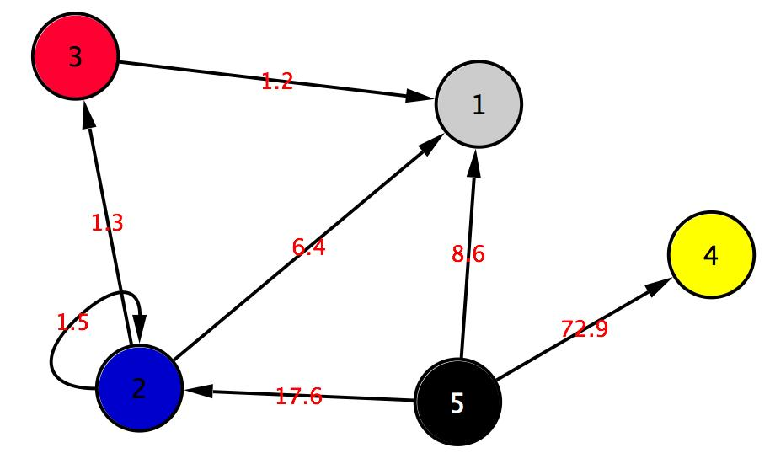
\epsfig{file=/ENSEIGN/COURS/MELANGE/Exposes/Figures/VEMmetagraphe.ps,
      width=.45\textwidth, clip=}  
      \\ \\
      \tiny{$\begin{array}{cccccc}
          \widehat{\gamma}_{k\ell}~(\%) & 1 & 2 & 3 & 4 & 5 \\
          \hline
          1 & . & . & . & . & . \\
          2 & 6.40 & 1.50 & 1.34 & . & . \\
          3 & 1.21 & . & . & . & . \\
          4 & . & . & . & . & . \\
          5 & 8.64 & 17.65 & . & 72.87 & 11.01 \\
          \hline
          \widehat{\alpha}~(\%) & 65.49 & 5.18 & 7.92 & 21.10 & 0.30
        \end{array}$}
      \\ \\
      (source \refer{PMD09})
    \end{tabular}
  \end{tabular}
  }

%====================================================================
%====================================================================
\section*{Variational Bayes inference}
\subsection*{Bayesian inference}
\frame{ \frametitle{Variational Bayes inference} \pause
%==================================================================== 
  \paragraph{Bayesian point of view:} The parameter $\thetabf$ itself
  {is random}:
  $$ 
  \thetabf \sim P(\thetabf)
  $$
  where $P(\thetabf)$ is {prior} distribution of $\thetabf$.

  \bigskip
  \paragraph{Bayesian inference:} The goal is then to calculate the
  {posterior} distribution
  $$
  P(\thetabf|\Xbf) = \frac{P(\thetabf) P(\Xbf|\thetabf)}{P(\Xbf)}.
  $$
  \begin{itemize}
  \item Its explicit calculation is possible in nice cases, e.g.
    exponential family with conjugate prior.
  \item Monte-Carlo (e.g. MCMC) sampling is often used to estimate it.
  \end{itemize}
  }

%==================================================================== 
\frame{\frametitle{Incomplete data model}
  \paragraph{Hierarchical modelling:} The model is typically defined
  with:
  $$
  \begin{tabular}{ll}
    the prior distribution of $\thetabf$: & \emphase{$P(\thetabf)$} \\
    \\
    the conditional distribution of the unobserved $\Zbf$: &
    \emphase{$P(\Zbf|\thetabf)$} \\
    \\
    the conditional distribution of the observed $\Xbf$: &
    \emphase{$P(\Xbf|\Zbf, \thetabf)$}
  \end{tabular}
  $$

  \bigskip
  \paragraph{Inference:} The goal is know to calculate (or estimate)
  the {joint conditional distribution}
  $$
  P(\Zbf, \thetabf|\Xbf) = \frac{P(\thetabf) P(\Zbf|\thetabf)
    P(\Xbf|\Zbf, \thetabf)}{P(\Xbf)}
  $$
  which is often {intractable}, even when $P(\Zbf|\Xbf,
  \thetabf)$ can be calculated (e.g. independent mixture models).
  }

%==================================================================== 
\subsection*{VB-EM}
%==================================================================== 
\frame{ \frametitle{Variational Bayes inference}
  \paragraph{Exponential family / conjugate prior:} if
  \begin{eqnarray*}
    \log P(\thetabf) & = & \phi(\thetabf)^\intercal \nubf + \cst \\
    \log P(\Xbf, \Zbf | \thetabf) & = & \phi(\thetabf)^\intercal
    u(\Xbf, \Zbf) + \cst. 
  \end{eqnarray*}

  \bigskip
  \paragraph{Variational optimisation:} The best approximate distribution
  $$
  Q^* = \arg\min_{Q \in \Qcal} KL[Q(\Zbf, \thetabf); P(\Zbf,
  \thetabf | \Xbf)]
  $$
  within the class of \emphase{factorisable distributions} $\Qcal$:
  $$
  \Qcal = \{Q: Q(\Zbf, \thetabf) = Q_Z(\Zbf)Q_\theta(\thetabf)\}
  $$
  can be recovered via a {variational Bayes E-M algorithm (VBEM)}
  [\refer{BeG03}]. 
}

%==================================================================== 
\frame{ \frametitle{VB-EM algorithm} 
  
  The approximate conditional distributions $Q_Z(\Zbf)$ and
  $Q_\theta(\thetabf)$ are alternatively updated.

  \paragraph{VB-M step:} Approximate posterior of $\thetabf$
  $$
  \log Q(\thetabf) = \phi(\thetabf)^\intercal \left\{\Esp_{Q_Z}[u(\Xbf,
    \Zbf)] + \nubf\right\} + \cst
  $$
  \paragraph{VB-E step:} Approximate conditional distribution of $\Zbf$
  $$
  \log Q(\Zbf) = \Esp_{Q_\theta}[\phi(\thetabf)]^\intercal u(\Xbf,
  \Zbf) + \cst
  $$

  \bigskip
  \paragraph{General properties:} Still not well known
  \begin{itemize}
  \item Consistency for some particular cases.
  \item Generally tend to underestimate the posterior variance of
    $\thetabf$.
  \item Obviously depends on the quality of the approximate
    $Q(\thetabf, \Zbf)$.
  \end{itemize}
  }

%==================================================================== 
\subsection*{Mixture for networks}
%==================================================================== 
\frame{ \frametitle{Application to mixtures for networks}
  \paragraph{VB-EM Credibility intervals} with a mixture of 2 groups of nodes\\
  ~\\
  \includegraphics[width=1\textwidth]{/ENSEIGN/COURS/MELANGE/Exposes/Figures/im-ICQ2-2-new} \\
  $\pi_1$: $+$, $\gamma_{11}$: \textcolor{red}{$\triangle$},
  $\gamma_{12}$: \textcolor{blue}{$\circ$}, $\gamma_{22}$:
  \textcolor{green}{$\bullet$}

  \begin{itemize}
  \item For all parameters, VB-EM posterior credibility intervals
    achieve the nominal level (90\%), as soon as $n \geq 25$.
  \item \emphase{$\rightarrow$} the VB-EM approximation works well, at least for
    graphs.
  \end{itemize}
  }

%====================================================================
\frame{ \frametitle{Approximate posterior distribution}
%==================================================================== 
  \vspace{-1cm}\hspace{-.5cm}
  \begin{tabular}{cc}
    \begin{tabular}{c}
      \includegraphics[width=.5\textwidth]{/ENSEIGN/COURS/MELANGE/Exposes/Figures/im-pi1BVEM}\\         
      \includegraphics[width=.5\textwidth]{/ENSEIGN/COURS/MELANGE/Exposes/Figures/im-pi2BVEM}\\
      \includegraphics[width=.5\textwidth]{/ENSEIGN/COURS/MELANGE/Exposes/Figures/im-pi3BVEM}\\
      \includegraphics[width=.5\textwidth]{/ENSEIGN/COURS/MELANGE/Exposes/Figures/im-pi4BVEM}\\
      \includegraphics[width=.5\textwidth]{/ENSEIGN/COURS/MELANGE/Exposes/Figures/im-pi5BVEM}\\
      \hline \\
      \includegraphics[width=.5\textwidth]{/ENSEIGN/COURS/MELANGE/Exposes/Figures/im-alphaBVEM}\\
    \end{tabular}
    &
    \begin{tabular}{c}
      \hspace{-.5cm}
      \includegraphics[width=.5\textwidth]{/ENSEIGN/COURS/MELANGE/Exposes/Figures/im_EcoliBVEM} \\
    \end{tabular}
  \end{tabular}  
  }



%%% Local Variables: 
%%% mode: latex
%%% TeX-master: "NeMo-SeMoVi"
%%% End: 
